\documentclass[12pt,a4paper]{report}

% =========================
% PACKAGES
% =========================
\usepackage[utf8]{inputenc}
\usepackage[T1]{fontenc}
\usepackage{geometry}
\usepackage{graphicx}
\usepackage{amsmath, amssymb}
\usepackage{hyperref}
\usepackage{listings}
\usepackage{xcolor}
\usepackage{booktabs}
\usepackage{fancyhdr}
\usepackage{tikz}
\usepackage{titlesec}
\usepackage{caption}

% =========================
% PAGE STYLE AND GEOMETRY
% =========================
\geometry{margin=1in}
\setlength{\headheight}{15pt} % ✅ Fix for fancyhdr warning
\pagestyle{fancy}
\fancyhf{}
\fancyhead[L]{\leftmark}
\fancyhead[R]{\thepage}
\renewcommand{\headrulewidth}{0.4pt}

% =========================
% TITLE FORMAT
% =========================
\titleformat{\chapter}[display]
  {\normalfont\bfseries\Huge}
  {\filleft\MakeUppercase{\chaptertitlename}~\thechapter}
  {2ex}
  {\titlerule\vspace{2ex}\filright}

% =========================
% CODE STYLE
% =========================
\lstdefinestyle{mystyle}{
    backgroundcolor=\color{gray!10},
    commentstyle=\color{teal},
    keywordstyle=\color{blue!90!black},
    numberstyle=\tiny\color{gray},
    stringstyle=\color{orange!90!black},
    basicstyle=\ttfamily\footnotesize,
    breaklines=true,
    numbers=left,
    numbersep=5pt,
    frame=single,
    captionpos=b
}
\lstset{style=mystyle}

% =========================
% CUSTOM COMMAND
% =========================
\newcommand{\vect}[1]{\boldsymbol{#1}}

% =========================
% DOCUMENT
% =========================
\begin{document}

\begin{titlepage}
    \centering
    {\Huge \textbf{Complex LaTeX Report Example}}\\[1.5cm]
    {\Large Mansoor Khan}\\[0.5cm]
    {\large Department of Computer Science}\\[0.5cm]
    {\large \today}\\[3cm]
    \includegraphics[width=0.3\textwidth]{example-image}\\[1cm]
    \vfill
    \textbf{Abstract:} \\
    This report demonstrates a complex LaTeX setup including equations, figures, code listings, and references — all suitable for Overleaf.
\end{titlepage}

\tableofcontents
\newpage

\chapter{Introduction}

LaTeX is a powerful typesetting system used for academic, technical, and scientific writing. This document showcases complex features such as mathematical equations, TikZ diagrams, and custom commands.

\section{Background}
Overleaf provides an online collaborative environment for writing LaTeX documents.

\section{Mathematical Example}
Here's an example of a mathematical expression:

\begin{equation}
    E = mc^2
\end{equation}

and a vector equation using our custom command:

\[
\vect{F} = m \cdot \vect{a}
\]

\chapter{Data and Figures}

\section{Table Example}
\begin{table}[ht] % ✅ fixed from [h!] to [ht]
\centering
\caption{Example Data Table}
\begin{tabular}{@{}lcc@{}}
\toprule
\textbf{Name} & \textbf{Score} & \textbf{Grade} \\
\midrule
Alice & 88 & B+ \\
Bob & 93 & A \\
Charlie & 76 & C \\
\bottomrule
\end{tabular}
\end{table}

\section{TikZ Diagram}
\begin{center}
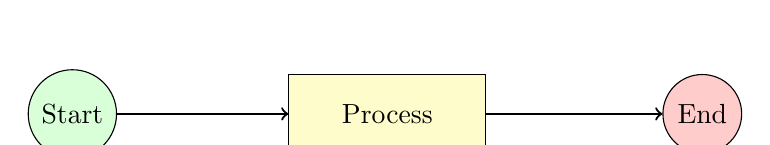
\begin{tikzpicture}[node distance=2.5cm, auto]
  \node (start) [circle, draw, fill=green!15, minimum size=1cm] {Start};
  \node (process) [rectangle, draw, fill=yellow!20, right of=start, node distance=4cm, minimum width=2.5cm, minimum height=1cm] {Process};
  \node (end) [circle, draw, fill=red!20, right of=process, node distance=4cm, minimum size=1cm] {End};
  \draw[->, thick] (start) -- (process);
  \draw[->, thick] (process) -- (end);
\end{tikzpicture}
\end{center}

\section{Including an Image}
\begin{figure}[ht] % ✅ fixed from [h!] to [ht]
\centering
\includegraphics[width=0.6\textwidth]{example-image-a}
\caption{Sample Placeholder Image}
\end{figure}

\chapter{Code Example}

\section{Python Code Listing}
\begin{lstlisting}[language=Python, caption=Simple Python Example]
def factorial(n):
    """Compute factorial using recursion."""
    if n == 0:
        return 1
    else:
        return n * factorial(n - 1)

print(factorial(5))
\end{lstlisting}

\chapter{Conclusion}

In this example, we explored how to combine mathematical expressions, figures, code snippets, and diagrams in a single LaTeX report. This serves as a strong starting point for academic reports or technical documentation.

\begin{thebibliography}{9}
\bibitem{latexcompanion}
  M. Goossens, F. Mittelbach, and A. Samarin,
  \textit{The LaTeX Companion},
  Addison-Wesley, 1993.

\bibitem{overleaf}
  Overleaf,
  \textit{LaTeX Documentation and Tutorials},
  \url{https://www.overleaf.com/learn}
\end{thebibliography}

\end{document}
